% case name
\chapter{convergence}

\section{Purpose}
The purpose of this example is to test the framework for automatic 
convergence studies.

\section{Description}
It consists of a schematic case with an analytical solution. 
It only involves the diffusion of a tracer so that the convergence study
measures the error done on the resolution of the time-discretised 
tracer equation:
\begin{equation}
\dfrac{T^{n+1} - T^{n}}{\Delta t} = -K \nabla^2 T^{n+1}
\end{equation}
where $K$ is the coefficient of diffusion for the tracer 
and $\Delta t$ is the time-step size.

\subsection{Geometry and mesh}
The case consists of a square basin of side $L=200m$. 
The coarse mesh contains 40 elements, it will be refined 4 times.
The mesh for each simulation and the mesh for
the error calculation are shown in the Figure \ref{fig:figure1}.

\begin{figure}
  \begin{center}
    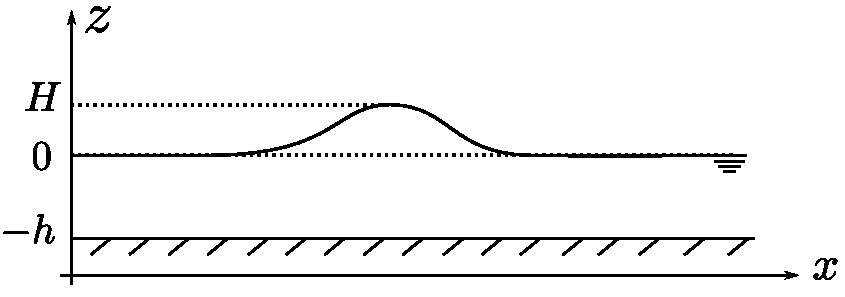
\includegraphics[scale=0.49]{img/figure1.pdf}
    \caption{Test on a schematic case: view of the meshes for each simulation
    -- (a) initial mesh, (c), (d), (e) successive refinements and 
    of the mesh for the error calculation (b).}
    \label{fig:figure1}
  \end{center}
\end{figure}

\subsection{Initial and boundary conditions}
The water height is constant and equal to $2m$ and the velocity 
is equal to zero.
The tracer is initialised with:
\begin{equation}
T = \left(1 - \dfrac{2 K}{\Delta t}\left(\dfrac{2 \pi}{L}\right)^2 \right)
\sin \left(\dfrac{2 \pi}{L}x \right) 
\sin \left( \dfrac{2 \pi}{L}y\right)
\end{equation}

$K$ is taken equal to $1 m s^{-2}$ and $\Delta t$ equal to $1s$.

\subsection{Analytical solution}

After one time-step, the tracer should be equal to:
\begin{equation}
T = \sin \left(\dfrac{2 \pi}{L}x \right) \sin \left( \dfrac{2 \pi}{L}y\right)
\end{equation}

\subsection{Numerical parameters}
The solver accuracy for the tracer diffusion is set to $10^{-10}$.
The advection and diffusion of velocities are deactivated in the steering file.
The simulation is done for 1 iteration.


\section{Results}
We compare the numerical solution for the tracer 
to the analytical solution after one time-step.

Three refinement levels were asked for in the convergence study, yielding
four TELEMAC-2D simulations. 

The total time spent for the four successive runs is of $4s$ on one processor 
(only the diffusion matrix inversion for the tracer is performed, on one time-step).
Figure \ref{fig:figure2} shows the results of the convergence study, regarding
the $L_1$, $L_2$ and $L_{\infty}$ errors. For the three of them, a first order
convergence is obtained. For the simulation on the finest mesh, the error
is slightly higher than expected, probably due to the worsened aspect ratio
of the triangles after three refinements. 
\begin{figure}
  \begin{center}
    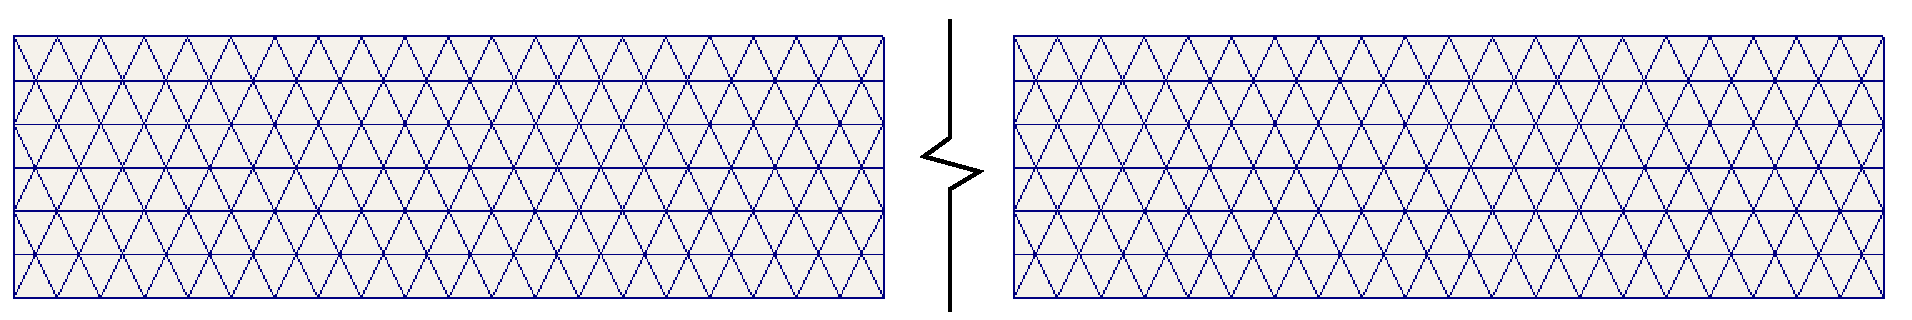
\includegraphics[scale=0.6]{img/figure2.pdf}
    \caption{Test on a schematic case: results of the convergence study
      with three refinement levels.}
    \label{fig:figure2}
  \end{center}
\end{figure}
